\documentclass{article}

\usepackage{tikz} 
\usetikzlibrary{automata, positioning, arrows, trees} 

\usepackage{amsthm}
\usepackage{amsfonts}
\usepackage{amsmath}
\usepackage{amssymb}
\usepackage{fullpage}
\usepackage{color}
\usepackage{parskip}
\usepackage{hyperref}

\usepackage{booktabs}

  \hypersetup{
    colorlinks = true,
    urlcolor = blue,       % color of external links using \href
    linkcolor= blue,       % color of internal links 
    citecolor= blue,       % color of links to bibliography
    filecolor= blue,       % color of file links
    }
    
\usepackage{listings}
\usepackage[utf8]{inputenc}                                                    
\usepackage[T1]{fontenc}
\usepackage{newunicodechar}
\newunicodechar{ℕ}{\ensuremath{\mathbb{N}}}                                                       

\definecolor{dkgreen}{rgb}{0,0.6,0}
\definecolor{gray}{rgb}{0.5,0.5,0.5}
\definecolor{mauve}{rgb}{0.58,0,0.82}

\lstset{frame=tb,
  language=haskell,
  aboveskip=3mm,
  belowskip=3mm,
  showstringspaces=false,
  columns=flexible,
  basicstyle={\small\ttfamily},
  numbers=none,
  numberstyle=\tiny\color{gray},
  keywordstyle=\color{blue},
  commentstyle=\color{dkgreen},
  stringstyle=\color{mauve},
  breaklines=true,
  breakatwhitespace=true,
  tabsize=3
}

\newtheoremstyle{theorem}
  {\topsep}   % ABOVESPACE
  {\topsep}   % BELOWSPACE
  {\itshape\/}  % BODYFONT
  {0pt}       % INDENT (empty value is the same as 0pt)
  {\bfseries} % HEADFONT
  {.}         % HEADPUNCT
  {5pt plus 1pt minus 1pt} % HEADSPACE
  {}          % CUSTOM-HEAD-SPEC
\theoremstyle{theorem} 
   \newtheorem{theorem}{Theorem}[section]
   \newtheorem{corollary}[theorem]{Corollary}
   \newtheorem{lemma}[theorem]{Lemma}
   \newtheorem{proposition}[theorem]{Proposition}
\theoremstyle{definition}
   \newtheorem{definition}[theorem]{Definition}
   \newtheorem{example}[theorem]{Example}
\theoremstyle{remark}    
  \newtheorem{remark}[theorem]{Remark}

\title{CPSC-354 Report}
\author{Nathan Garcia  \\ Chapman University}

\date{\today} 

\begin{document}

\maketitle

\begin{abstract}
\end{abstract}

\setcounter{tocdepth}{3}
\tableofcontents

\section{Introduction}\label{intro}

The report contains all homework assignments which students completed during one semester of CPSC-354 (Programming Languages) at Chapman University. The collection includes all weekly work from Weeks 1 through 13 which includes assignments and proofs and derivations and small programming tasks that demonstrate fundamental concepts of programming languages and formal reasoning.

\paragraph{Brief Overview.}
\begin{itemize}
  \item Core topics: abstract rewriting systems, invariants, termination measures, lambda calculus (\(\alpha/\beta\)-reduction, fixed points), Church numerals, and simple interpreters.
  \item Syntax and parsing: grammar-based derivations and parse trees; operator precedence and the role of parentheses.
  \item Proof practice: algebraic laws (associativity, commutativity), propositional logic, and Lean-based proofs.
  \item Algorithms and traces: Euclid's GCD, merge sort measures, and Towers of Hanoi execution with move sequences.
\end{itemize}

\paragraph{Structure.}
The ``Week by Week'' section organizes each homework with consistent naming (Week \(n\), HW \(n\)) and concise expositions, including diagrams, equations, or code where appropriate.

\section{Week by Week}\label{homework}

\subsection{Week 1}
\subsubsection{HW 1 - MU Puzzle}

The MU puzzle comes from the book \textit{Gödel, Escher, Bach}. You start with the string \textbf{MI} and the goal is to turn it into \textbf{MU} by following four rules:

\begin{enumerate}
    \item If a string ends with \textbf{I}, you can add a \textbf{U} at the end.  
    \item If a string starts with \textbf{M}, you can copy everything after the M.  
    \item If you see \textbf{III}, you can change it to \textbf{U}.  
    \item If you see \textbf{UU}, you can delete it.  
\end{enumerate}

The puzzle is about seeing if you can reach \textbf{MU} by only using these rules. It is not really about the letters themselves, but about how rules control what strings you can or cannot make.
\subsubsection{HW 1b - MU Puzzle Analysis}

The MU puzzle comes from the book \textit{Gödel, Escher, Bach}. You start with the string \textbf{MI} and the goal is to turn it into \textbf{MU} by following four rules:

\begin{enumerate}
    \item If a string ends with \textbf{I}, you can add a \textbf{U} at the end.  
    \item If a string starts with \textbf{M}, you can copy everything after the M.  
    \item If you see \textbf{III}, you can change it to \textbf{U}.  
    \item If you see \textbf{UU}, you can delete it.  
\end{enumerate}

At first, I tried small derivations. For example:
\[
\texttt{MI} \;\Rightarrow\; \texttt{MIU} \;\Rightarrow\; \texttt{MIUIU}
\]
or duplicating I’s:
\[
\texttt{MI} \;\Rightarrow\; \texttt{MII} \;\Rightarrow\; \texttt{MIIII}
\]
From \texttt{MIIII}, I can replace \texttt{III} with \texttt{U}, giving \texttt{MUI}, but not \texttt{MU}. Every time, an extra \texttt{I} is left over, and there is no rule that deletes a single \texttt{I}.

\paragraph{Invariant Argument.}  
Let $\#I(w)$ denote the number of \texttt{I}'s in string $w$. If we track $\#I(w) \pmod 3$, we find:
\begin{itemize}
    \item Rule 1: $\#I$ unchanged.  
    \item Rule 2: $\#I$ doubles. Over $\mathbb{Z}/3\mathbb{Z}$, $1 \mapsto 2$, $2 \mapsto 1$, never $0$.  
    \item Rule 3: Removes $3$ I’s, leaving the remainder mod 3 unchanged.  
    \item Rule 4: Deletes U’s only, so $\#I$ unchanged.  
\end{itemize}

We start with \texttt{MI}, which has $\#I=1$. This is congruent to $1 \pmod 3$. Because no rule ever makes $\#I \equiv 0 \pmod 3$, it is impossible to reach a string with $\#I=0$.

\paragraph{Conclusion.}  
The target \texttt{MU} has $\#I=0$, which is divisible by $3$. Since that is unreachable from \texttt{MI}, the puzzle is unsolvable. As a student, the cool part here is that the solution isn’t about brute-force trying rules—it’s about spotting a hidden invariant (the number of I’s mod 3) that blocks the path completely.

\subsection{Week 2}
\subsubsection{HW 2 - Abstract Rewriting Systems (ARS) Properties}

\paragraph{Problem.}
Consider the following list of Abstract Rewriting Systems (ARSs).
\begin{enumerate}
  \item $A=\varnothing$.
  \item $A=\{a\}$ \; and \; $R=\varnothing$.
  \item $A=\{a\}$ \; and \; $R=\{(a,a)\}$.
  \item $A=\{a,b,c\}$ \; and \; $R=\{(a,b),(a,c)\}$.
  \item $A=\{a,b\}$ \; and \; $R=\{(a,a),(a,b)\}$.
  \item $A=\{a,b,c\}$ \; and \; $R=\{(a,b),(b,b),(a,c)\}$.
  \item $A=\{a,b,c\}$ \; and \; $R=\{(a,b),(b,b),(a,c),(c,c)\}$.
\end{enumerate}

\noindent\textbf{Task.} Draw a picture for each ARS above (nodes = elements of $A$, arrows = pairs in $R$).
Then determine whether each ARS is \emph{terminating}, \emph{confluent}, and whether it has \emph{unique normal forms}.

% ---------- STYLE FOR ALL DIAGRAMS ----------
\tikzset{
  rsnode/.style = {circle, draw, minimum size=7mm, inner sep=0pt},
  rsgraph/.style = {->, thick, node distance=2.0cm}
}

\medskip

% ===== ARS 1 =====
\begin{center}
\begin{tikzpicture}[rsgraph]
  % A = empty set -> no nodes, just a label
  \node[draw=none] (lab) {\textbf{ARS 1:} $A=\varnothing$ (no elements to draw)};
\end{tikzpicture}
\end{center}

% ===== ARS 2 =====
\begin{center}
\begin{tikzpicture}[rsgraph]
  % A = {a}, R = empty (just one isolated node, no arrows)
  \node[rsnode] (a) {a};
  \node[draw=none, below=8pt of a] { \textbf{ARS 2:} $A=\{a\},\ R=\varnothing$ };
\end{tikzpicture}
\end{center}

% ===== ARS 3 =====
\begin{center}
\begin{tikzpicture}[rsgraph]
  % A = {a}, R = {(a,a)}  -- single node with a self-loop
  \node[rsnode] (a) {a};
  \path (a) edge[loop right] (a);
\end{tikzpicture}

\smallskip
\textbf{ARS 3:} $A=\{a\},\ R=\{(a,a)\}$
\end{center}


% ===== ARS 4 =====
\begin{center}
\begin{tikzpicture}[rsgraph]
  % A = {a,b,c}, R = {(a,b),(a,c)}
  \node[rsnode] (a) {a};
  \node[rsnode, below left=1.2cm and 1.2cm of a] (b) {b};
  \node[rsnode, below right=1.2cm and 1.2cm of a] (c) {c};
  \path (a) edge (b)
        (a) edge (c);
  \node[draw=none, below=8pt of b.center, xshift=1.2cm] { \textbf{ARS 4:} $A=\{a,b,c\},\ R=\{(a,b),(a,c)\}$ };
\end{tikzpicture}
\end{center}

% ===== ARS 5 =====
\begin{center}
\begin{tikzpicture}[rsgraph]
  % A = {a,b}, R = {(a,a),(a,b)}
  \node[rsnode] (a) {a};
  \node[rsnode, right=2.5cm of a] (b) {b};
  \path (a) edge[loop above] (a)
        (a) edge (b);
  \node[draw=none, below=8pt of a, xshift=1.25cm] { \textbf{ARS 5:} $A=\{a,b\},\ R=\{(a,a),(a,b)\}$ };
\end{tikzpicture}
\end{center}

% ===== ARS 6 =====
\begin{center}
\begin{tikzpicture}[rsgraph]
  % A = {a,b,c}, R = {(a,b),(b,b),(a,c)}
  \node[rsnode] (a) {a};
  \node[rsnode, below left=1.2cm and 1.2cm of a] (b) {b};
  \node[rsnode, below right=1.2cm and 1.2cm of a] (c) {c};
  \path (a) edge (b)
        (a) edge (c)
        (b) edge[loop left] (b);
  \node[draw=none, below=8pt of b.center, xshift=1.2cm] { \textbf{ARS 6:} $A=\{a,b,c\},\ R=\{(a,b),(b,b),(a,c)\}$ };
\end{tikzpicture}
\end{center}

% ===== ARS 7 =====
\begin{center}
\begin{tikzpicture}[rsgraph]
  % A = {a,b,c}, R = {(a,b),(b,b),(a,c),(c,c)}
  \node[rsnode] (a) {a};
  \node[rsnode, below left=1.2cm and 1.2cm of a] (b) {b};
  \node[rsnode, below right=1.2cm and 1.2cm of a] (c) {c};
  \path (a) edge (b)
        (a) edge (c)
        (b) edge[loop left] (b)
        (c) edge[loop right] (c);
  \node[draw=none, below=8pt of b.center, xshift=1.2cm] { \textbf{ARS 7:} $A=\{a,b,c\},\ R=\{(a,b),(b,b),(a,c),(c,c)\}$ };
\end{tikzpicture}
\end{center}


\begin{center}
\begin{tabular}{@{}lccc@{}}
\toprule
\textbf{ARS} & \textbf{Terminating} & \textbf{Confluent} & \textbf{Has Unique Normal Forms} \\
\midrule
1 & \phantom{True/False}X & \phantom{True/False}X & \phantom{True/False}X \\
2 & X & X & X \\
3 &  & X &  \\
4 & X &  & X \\
5 &  & X & X \\
6 &  &  &  \\
7 &  &  &  \\
\bottomrule
\end{tabular}
\end{center}
\begin{enumerate}
  \item \textbf{Confluent: True}, \textbf{Terminating: True}, \textbf{Unique Normal Forms: False}\\
  % This is not possible
  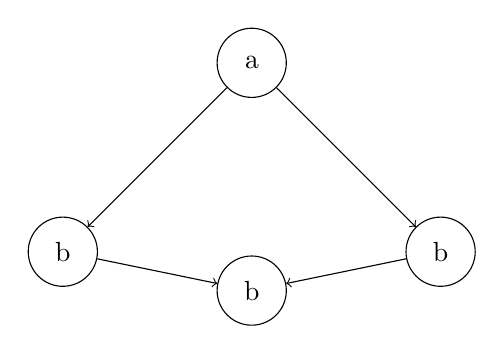
\begin{tikzpicture}[->, node distance=2.5cm]
    \node[state] (a) {a};
    \node[state, below left=of a] (b1) {b};
    \node[state, below right=of a] (b2) {b};
    \node[state, below=2cm of a] (b3) {b};
    \draw (a) -- (b1);
    \draw (a) -- (b2);
    \draw (b1) -- (b3);
    \draw (b2) -- (b3);
  \end{tikzpicture}

  \item \textbf{Confluent: True}, \textbf{Terminating: False}, \textbf{Unique Normal Forms: True}\\
  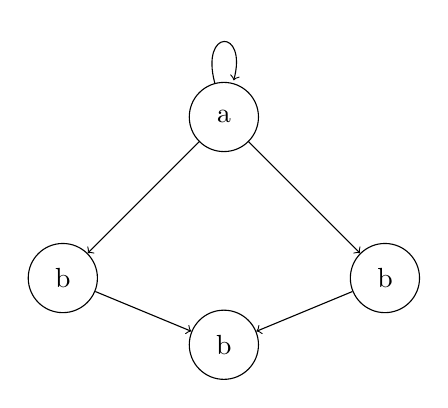
\begin{tikzpicture}[->, node distance=2cm]
    \node[state] (a) {a};
    \node[state, below left=of a] (b1) {b};
    \node[state, below right=of a] (b2) {b};
    \node[state, below=2cm of a] (b3) {b};
    \draw (a) -- (b1);
    \draw (a) -- (b2);
    \draw (b1) -- (b3);
    \draw (b2) -- (b3);
    \draw (a) edge[loop above] (a);
  \end{tikzpicture}

  \item \textbf{Confluent: True}, \textbf{Terminating: False}, \textbf{Unique Normal Forms: False}\\
  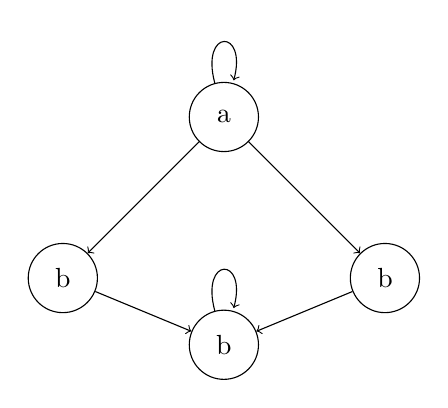
\begin{tikzpicture}[->, node distance=2cm]
    \node[state] (a) {a};
    \node[state, below left=of a] (b1) {b};
    \node[state, below right=of a] (b2) {b};
    \node[state, below=2cm of a] (b3) {b};
    \draw (a) -- (b1);
    \draw (a) -- (b2);
    \draw (b1) -- (b3);
    \draw (b2) -- (b3);
    \draw (a) edge[loop above] (a);
    \draw (b3) edge[loop above] (b3);
  \end{tikzpicture}

  \item \textbf{Confluent: False}, \textbf{Terminating: True}, \textbf{Unique Normal Forms: True}\\
  \begin{tikzpicture}[->, node distance=2cm]
    \node[state] (a) {a};
    \node[state, below right=of a] (b) {b};
    \draw (a) -- (b);
  \end{tikzpicture}

  \item \textbf{Confluent: False}, \textbf{Terminating: True}, \textbf{Unique Normal Forms: False}\\
  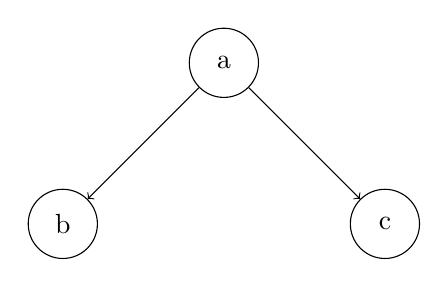
\begin{tikzpicture}[->, node distance=2cm]
    \node[state] (a) {a};
    \node[state, below left=of a] (b) {b};
    \node[state, below right=of a] (c) {c};
    \draw (a) -- (b);
    \draw (a) -- (c);
  \end{tikzpicture}

  \item \textbf{Confluent: False}, \textbf{Terminating: False}, \textbf{Unique Normal Forms: True}\\
  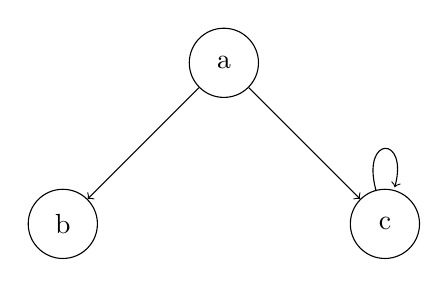
\begin{tikzpicture}[->, node distance=2cm]
    \node[state] (a) {a};
    \node[state, below left=of a] (b) {b};
    \node[state, below right=of a] (c) {c};
    \draw (a) -- (b);
    \draw (a) -- (c);
    \draw (c) edge[loop above] (c);
  \end{tikzpicture}

  \item \textbf{Confluent: False}, \textbf{Terminating: False}, \textbf{Unique Normal Forms: False}\\
  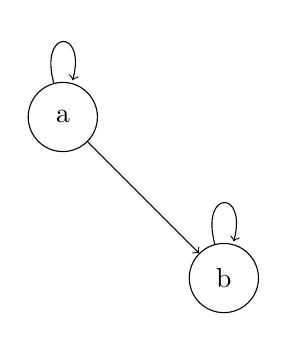
\begin{tikzpicture}[->, node distance=2cm]
    \node[state] (a) {a};
    \node[state, below right=of a] (b) {b};
    \draw (a) -- (b);
    \draw (a) edge[loop above] (a);
    \draw (b) edge[loop above] (b);
  \end{tikzpicture}
\end{enumerate}

\subsection{Week 3}
\subsubsection{HW 3 - Exercise 5: Reduction}
\textbf{Exercise 5.}

\textit{Rules:}
\[
ab \to ba, \quad ba \to ab, \quad aa \to \epsilon, \quad b \to \epsilon
\]

\textit{Sample reductions:}
\[
abba \;\to\; bbaa \;\to\; baa \;\to\; aa \;\to\; \epsilon
\]
\[
bababa \;\to\; aaabbb \;\to\; aabbb \;\to\; abbb \;\to\; a
\]

\textit{Non-termination:} The rules $ab \to ba$ and $ba \to ab$ form an infinite loop:
\[
ab \to ba \to ab \to ba \to \cdots
\]

\textit{Non-equivalent strings:} $a$ and $\epsilon$ are not equivalent, since a single $a$ cannot be eliminated.

\textit{Equivalence classes:}  
Order does not matter (due to swapping).  
$b$’s vanish.  
$aa \to \epsilon$ ensures only the \emph{parity} of the number of $a$’s matters.  

\[
I(w) = \#a(w) \bmod 2 \in \{0,1\}
\]

Thus there are exactly two equivalence classes:
\[
\{w \mid \#a(w) \equiv 0 \pmod 2\} \quad\longmapsto\quad \epsilon
\]
\[
\{w \mid \#a(w) \equiv 1 \pmod 2\} \quad\longmapsto\quad a
\]

\textit{Modified terminating system:}
\[
ab \to ba, \quad aa \to \epsilon, \quad b \to \epsilon
\]
Termination follows from length and inversion-count measures.  

\textit{Specification:} The algorithm computes the \emph{parity of the number of $a$’s}, ignoring $b$’s.

\vspace{1em}

\textbf{Exercise 5b.}

\textit{Rules:}
\[
ab \to ba, \quad ba \to ab, \quad aa \to a, \quad b \to \epsilon
\]

\textit{Sample reductions:}
\[
abba \;\to\; bbaa \;\to\; baa \;\to\; aa \;\to\; a
\]
\[
bababa \;\to\; aaabbb \;\to\; aabbb \;\to\; abbb \;\to\; a
\]

\textit{Non-termination:} As before, infinite swapping is possible.

\textit{Non-equivalent strings:} $\epsilon$ and $a$ are not equivalent: all $b$’s vanish, and any positive number of $a$’s reduces to $a$.

\textit{Equivalence classes:}  
Order does not matter.  
$b$’s vanish.  
$aa \to a$ collapses any positive number of $a$’s to a single $a$.  

\[
J(w) =
\begin{cases}
0 & \text{if } \#a(w) = 0 \\
1 & \text{if } \#a(w) \geq 1
\end{cases}
\]

Thus there are exactly two equivalence classes:
\[
\{w \mid \#a(w) = 0\} \quad\longmapsto\quad \epsilon
\]
\[
\{w \mid \#a(w) \geq 1\} \quad\longmapsto\quad a
\]

\textit{Modified terminating system:}
\[
ab \to ba, \quad aa \to a, \quad b \to \epsilon
\]
This terminates and yields unique normal forms.  

\textit{Specification:} The algorithm computes whether the input contains at least one $a$, ignoring all $b$’s.

\subsection{Week 4}
\subsubsection{HW 4 - Termination}

For the definition of a \emph{measure function}, see our notes on rewriting and, in particular, on termination.

\paragraph{HW 4.1.}
Consider the following algorithm (Euclid’s algorithm for the greatest common divisor):

\begin{verbatim}
while b != 0:
    temp = b
    b = a mod b
    a = temp
return a
\end{verbatim}

\textbf{Conditions.} Assume inputs $a,b \in \mathbb{N}$ with $b \geq 0$ and the usual remainder operation, i.e.\ for $b>0$ we have $0 \leq a \bmod b < b$. (If $b=0$, the loop is skipped and the algorithm terminates immediately.)

\textbf{Measure function.} Define
\[
\mu(a,b) := b \in \mathbb{N}.
\]

\textbf{Proof of termination.}  
If the loop guard holds ($b \neq 0$), one iteration maps the state $(a,b)$ to
\[
(a',b') = (\,b,\ a \bmod b\,).
\]
By the property of the remainder,
\[
0 \leq b' = a \bmod b < b = \mu(a,b).
\]
Thus $\mu$ strictly decreases on every loop iteration and is bounded below by $0$.  
Since $(\mathbb{N},<)$ is well-founded, no infinite descending chain
\[
\mu(a_0,b_0) > \mu(a_1,b_1) > \mu(a_2,b_2) > \cdots
\]
exists. Hence only finitely many iterations are possible; the loop terminates and the algorithm halts. \qed

\medskip

\paragraph{HW 4.2.}
Consider the following fragment of merge sort:

\begin{verbatim}
function merge_sort(arr, left, right):
    if left >= right:
        return
    mid = (left + right) / 2
    merge_sort(arr, left, mid)
    merge_sort(arr, mid+1, right)
    merge(arr, left, mid, right)
\end{verbatim}

Define
\[
\phi(left,right) := right - left + 1.
\]

\textbf{Claim.} $\phi$ is a measure function for \texttt{merge\_sort}.

\textbf{Proof.}
\begin{itemize}
    \item \emph{Well-defined, nonnegative.} For valid indices with $left \leq right$, we have $\phi(left,right) \in \mathbb{N}$ and $\phi \geq 1$. If $left > right$ the function is not called (or $\phi \leq 0$, and the base case applies immediately).
    \item \emph{Base case.} When $left \geq right$, the function returns immediately; in this case $\phi(left,right) \leq 1$, i.e.\ there is no further recursion.
    \item \emph{Strict decrease on recursive calls.} Suppose $left < right$ and let $n := \phi(left,right) = right-left+1 \geq 2$. With $mid = \lfloor (left+right)/2 \rfloor$:
    \[
    \phi(left,mid) = mid - left + 1 \leq \left\lfloor \tfrac{n}{2} \right\rfloor < n,
    \]
    \[
    \phi(mid+1,right) = right - (mid+1) + 1 = right - mid \leq \left\lceil \tfrac{n}{2} \right\rceil < n.
    \]
    Thus both recursive calls strictly reduce the measure.
\end{itemize}

Since $\phi$ maps each call to a natural number that strictly decreases along every recursive edge and is bounded below, there are no infinite descending chains. By well-founded induction on $\phi$, all recursive calls terminate. \qed

\subsection{Week 5}

\subsubsection{HW 5 - Workout: Step-by-step \texorpdfstring{$\alpha$/$\beta$}{alpha/beta}-reductions}

\noindent\textbf{Problem.} Evaluate
\[
(\lambda f.\,\lambda x.\,f(f\,x))\;(\lambda f.\,\lambda x.\,f(f(f\,x))).
\]

\noindent\textbf{Notation.}
We use $\rightsquigarrow_\beta$ for a single $\beta$-reduction step and “$\alpha$” to indicate a capture-avoiding renaming of bound variables.

\noindent\textbf{Intuition.}
The term $\lambda f.\,\lambda x.\,f(f\,x)$ applies a function twice (\emph{iterate-2}).  
The term $\lambda f.\,\lambda x.\,f(f(f\,x))$ applies a function three times (\emph{iterate-3}).  
Applying iterate-2 \emph{to} iterate-3 yields iterate-9.

\noindent\textbf{Derivation.}
\begin{align*}
&(\lambda f.\,\lambda x.\,f(f\,x))\;(\lambda f.\,\lambda x.\,f(f(f\,x)))\\[2pt]
&\rightsquigarrow_\beta\ \lambda x.\, \big[(\lambda f.\,\lambda x.\,f(f(f\,x)))\big((\lambda f.\,\lambda x.\,f(f(f\,x)))\,x\big)\big]
\quad\text{(substitute $f := \lambda f.\lambda x.\,f(f(f\,x))$ into $\lambda x.\,f(f\,x)$)}\\[4pt]
&\overset{\alpha}{=}\ \lambda x.\, (\lambda f.\,\lambda y.\,f(f(f\,y)))\Big((\lambda f.\,\lambda u.\,f(f(f\,u)))\,x\Big)
\quad\text{(rename bound $x$'s to $y,u$ to avoid shadowing)}\\[4pt]
&\rightsquigarrow_\beta\ \lambda x.\, (\lambda f.\,\lambda y.\,f(f(f\,y)))\big(\lambda u.\,x(x(x\,u))\big)
\quad\text{(apply $\beta$ to $(\lambda f.\lambda u.\,f(f(f\,u)))\,x$)}\\[4pt]
&\rightsquigarrow_\beta\ \lambda x.\,\lambda y.\,F\big(F(F\,y)\big)
\quad\text{with }F:=\lambda u.\,x(x(x\,u))
\quad\text{(apply $(\lambda f.\lambda y.\,f(f(f\,y)))\,F$)}\\[4pt]
&=\ \lambda x.\,\lambda y.\,F\Big(F\big(F\,y\big)\Big)\\[2pt]
&=\ \lambda x.\,\lambda y.\,F\Big(F\big(x(x(x\,y))\big)\Big)
\quad\text{(since $F\,y = x(x(x\,y))$)}\\[2pt]
&=\ \lambda x.\,\lambda y.\,F\Big(x\big(x\big(x\big(x(x(x\,y))\big)\big)\big)\Big)
\quad\text{(apply $F$ again; adds $3$ more $x$'s: total $6$)}\\[2pt]
&=\ \lambda x.\,\lambda y.\,x\big(x\big(x\big(x\big(x\big(x\big(x\big(x\big(x\,y\big)\big)\big)\big)\big)\big)\big)\big)
\quad\text{(apply $F$ a third time; +3 more: total $9$)}.
\end{align*}

\noindent\textbf{Normal form.}
\[
\boxed{\ \lambda x.\,\lambda y.\,\underbrace{x(x(x(x(x(x(x(x(x\,y))))))))}_{\text{$9$ applications of }x}\ }
\]
So the result is the \emph{iterate-9} operator: given $x$ and $y$, it applies $x$ to $y$ nine times.

\subsection{Week 6}
\subsubsection{HW 6 - Computing \texorpdfstring{$\mathrm{fact}\,3$}{fact 3} via a Fixed Point Combinator}

We use the computation rules
\[
\begin{aligned}
&\mathtt{fix}\ F \;\to\; (F\ (\mathtt{fix}\ F)) && \text{(fix)}\\
&\mathtt{let}\ x = e_1\ \mathtt{in}\ e_2 \;\to\; ((\lambda x.\, e_2)\ e_1) && \text{(let)}\\
&\mathtt{let\ rec}\ f = e_1\ \mathtt{in}\ e_2 \;\to\; \mathtt{let}\ f = (\mathtt{fix}\ (\lambda f.\, e_1))\ \mathtt{in}\ e_2 && \text{(let rec)}
\end{aligned}
\]
and the usual \(\beta\)-reduction \(((\lambda x.\,e)\ v) \to e[x:=v]\), plus base computation rules
\[
0=0\to \mathtt{True},\quad n{>}0 \Rightarrow (n=0)\to \mathtt{False},\quad
\mathtt{if}\ \mathtt{True}\ \mathtt{then}\ A\ \mathtt{else}\ B \to A,\quad
\mathtt{if}\ \mathtt{False}\ \mathtt{then}\ A\ \mathtt{else}\ B \to B.
\]

\paragraph{Abbreviation.}
Let
\[
F \;\equiv\; \lambda f.\,\lambda n.\,
\mathtt{if}\ (n=0)\ \mathtt{then}\ 1\ \mathtt{else}\ n * f(n-1).
\]
Then \(\mathtt{fact} \equiv \mathtt{fix}\ F\).

\paragraph{Goal.}
Evaluate
\[
\mathtt{let\ rec}\ \mathtt{fact} = \lambda n.\,\mathtt{if}\ (n=0)\ \mathtt{then}\ 1\ \mathtt{else}\ n * \mathtt{fact}(n-1)\ \mathtt{in}\ \mathtt{fact}\ 3.
\]

\begin{align*}
&\mathtt{let\ rec}\ \mathtt{fact}=\lambda n.\,\dots\ \mathtt{in}\ \mathtt{fact}\ 3\\
{}\to\;& \mathtt{let}\ \mathtt{fact}=(\mathtt{fix}\ (\lambda f.\,\lambda n.\,\dots))\ \mathtt{in}\ \mathtt{fact}\ 3
&&\text{(let rec)}\\
{}\to\;& ((\lambda \mathtt{fact}.\, \mathtt{fact}\ 3)\ (\mathtt{fix}\ F))
&&\text{(let)}\\
{}\to\;& (\mathtt{fix}\ F)\ 3
&&\text{(\(\beta\))}\\[4pt]
{}\to\;& (F\ (\mathtt{fix}\ F))\ 3
&&\text{(fix)}\\
{}\to\;& ((\lambda f.\,\lambda n.\,\mathtt{if}\ (n=0)\ \mathtt{then}\ 1\ \mathtt{else}\ n * f(n-1))\ (\mathtt{fix}\ F))\ 3
&&\text{(def.\ of \(F\))}\\
{}\to\;& (\lambda n.\,\mathtt{if}\ (n=0)\ \mathtt{then}\ 1\ \mathtt{else}\ n * (\mathtt{fix}\ F)(n-1))\ 3
&&\text{(\(\beta\))}\\
{}\to\;& \mathtt{if}\ (3=0)\ \mathtt{then}\ 1\ \mathtt{else}\ 3 * (\mathtt{fix}\ F)(2)
&&\text{(\(\beta\))}\\
{}\to\;& 3 * (\mathtt{fix}\ F)(2)
&&\text{(arith.\ and if-False)}
\end{align*}

Now expand \((\mathtt{fix}\ F)\ 2\):
\begin{align*}
(\mathtt{fix}\ F)2
&\to (F(\mathtt{fix}\ F))2 &&\text{(fix)}\\
&\to \mathtt{if}\ (2=0)\ \mathtt{then}\ 1\ \mathtt{else}\ 2 * (\mathtt{fix}\ F)(1)
&&\text{(def.\ \(F\), \(\beta\))}\\
&\to 2 * (\mathtt{fix}\ F)(1)
&&\text{(if-False)}
\end{align*}

Expand \((\mathtt{fix}\ F)1\):
\begin{align*}
(\mathtt{fix}\ F)1
&\to (F(\mathtt{fix}\ F))1 &&\text{(fix)}\\
&\to \mathtt{if}\ (1=0)\ \mathtt{then}\ 1\ \mathtt{else}\ 1 * (\mathtt{fix}\ F)(0)
&&\text{(def.\ \(F\), \(\beta\))}\\
&\to 1 * (\mathtt{fix}\ F)(0)
&&\text{(if-False)}
\end{align*}

Expand \((\mathtt{fix}\ F)0\):
\begin{align*}
(\mathtt{fix}\ F)0
&\to (F(\mathtt{fix}\ F))0 &&\text{(fix)}\\
&\to \mathtt{if}\ (0=0)\ \mathtt{then}\ 1\ \mathtt{else}\ 0 * (\mathtt{fix}\ F)(-1)
&&\text{(def.\ \(F\), \(\beta\))}\\
&\to 1
&&\text{(if-True)}
\end{align*}

Unwinding:
\[
1 * (\mathtt{fix}\ F)0 \to 1 * 1 \to 1,\qquad
2 * (\mathtt{fix}\ F)1 \to 2 * 1 \to 2,\qquad
3 * (\mathtt{fix}\ F)2 \to 3 * 2 \to 6.
\]

\[
\boxed{\ \mathtt{fact}\ 3 \;\to^{\!*}\; 6\ }
\]


\subsection{Week 7}
\subsubsection{HW 7 - Parse Trees for Arithmetic Expressions}

\textbf{Using the context-free grammar:}

\begin{verbatim}
Exp  -> Exp '+' Exp1
Exp1 -> Exp1 '*' Exp2
Exp2 -> Integer
Exp2 -> '(' Exp ')'
Exp  -> Exp1
Exp1 -> Exp2
\end{verbatim}

Write out the derivation trees (parse trees) for the following strings:

2+1,  1+2*3,  1+(2*3),  (1+2)*3,  1+2*3+4*5+6

---

\paragraph{1. Parse tree for 2 + 1}

\begin{center}
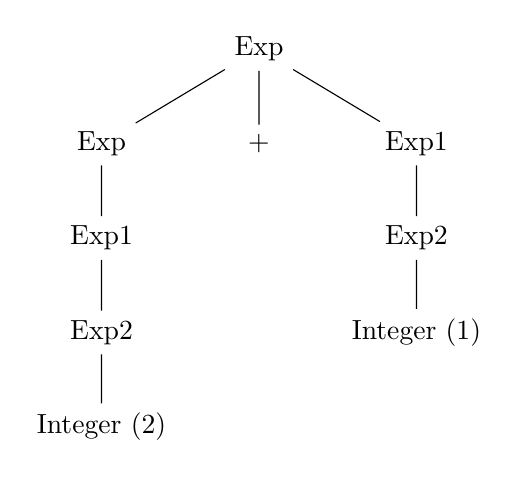
\begin{tikzpicture}[level distance=1.2cm, sibling distance=2cm]
\node {Exp}
  child {node {Exp}
    child {node {Exp1}
      child {node {Exp2}
        child {node {Integer (2)}}}}}
  child {node {$+$}}
  child {node {Exp1}
    child {node {Exp2}
      child {node {Integer (1)}}}};
\end{tikzpicture}
\end{center}

---

\paragraph{2. Parse tree for 1 + 2 * 3}

\begin{center}
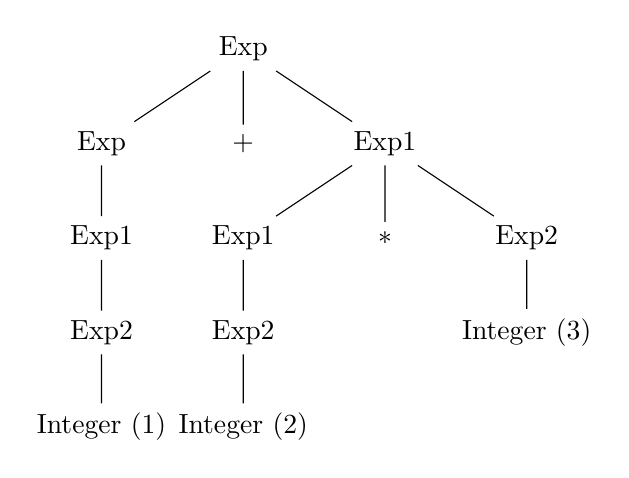
\begin{tikzpicture}[level distance=1.2cm, sibling distance=1.8cm]
\node {Exp}
  child {node {Exp}
    child {node {Exp1}
      child {node {Exp2}
        child {node {Integer (1)}}}}}
  child {node {$+$}}
  child {node {Exp1}
    child {node {Exp1}
      child {node {Exp2}
        child {node {Integer (2)}}}}
    child {node {$*$}}
    child {node {Exp2}
      child {node {Integer (3)}}}};
\end{tikzpicture}
\end{center}

---

\paragraph{3. Parse tree for 1 + (2 * 3)}

\begin{center}
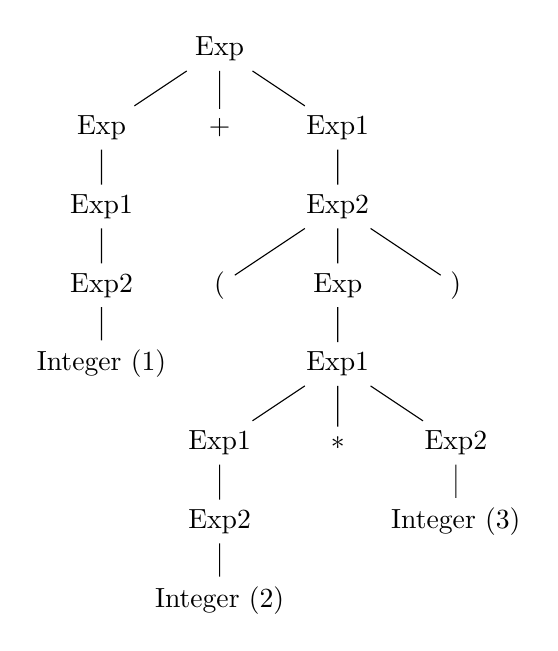
\begin{tikzpicture}[level distance=1.0cm, sibling distance=1.5cm]
\node {Exp}
  child {node {Exp}
    child {node {Exp1}
      child {node {Exp2}
        child {node {Integer (1)}}}}}
  child {node {$+$}}
  child {node {Exp1}
    child {node {Exp2}
      child {node {$($}}
      child {node {Exp}
        child {node {Exp1}
          child {node {Exp1}
            child {node {Exp2}
              child {node {Integer (2)}}}}
          child {node {$*$}}
          child {node {Exp2}
            child {node {Integer (3)}}}}}
      child {node {$)$}}}};
\end{tikzpicture}
\end{center}

---

\paragraph{4. Parse tree for (1 + 2) * 3}

\begin{center}
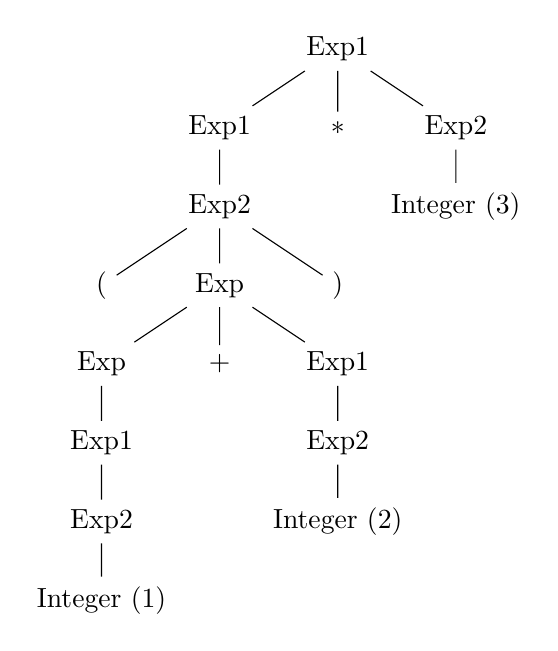
\begin{tikzpicture}[level distance=1.0cm, sibling distance=1.5cm]
\node {Exp1}
  child {node {Exp1}
    child {node {Exp2}
      child {node {$($}}
      child {node {Exp}
        child {node {Exp}
          child {node {Exp1}
            child {node {Exp2}
              child {node {Integer (1)}}}}}
        child {node {$+$}}
        child {node {Exp1}
          child {node {Exp2}
            child {node {Integer (2)}}}}}
      child {node {$)$}}}}
  child {node {$*$}}
  child {node {Exp2}
    child {node {Integer (3)}}};
\end{tikzpicture}
\end{center}

---

\paragraph{5. Parse tree for 1 + 2 * 3 + 4 * 5 + 6}

\begin{center}
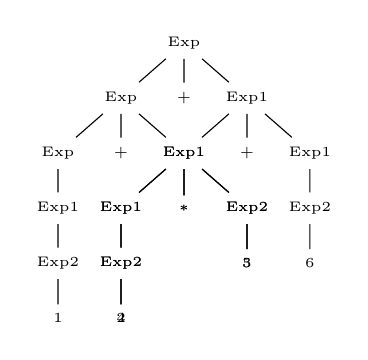
\begin{tikzpicture}[level distance=0.7cm, sibling distance=0.8cm, 
                    every node/.style={font=\tiny}]
\node {Exp}
  child {node {Exp}
    child {node {Exp}
      child {node {Exp1}
        child {node {Exp2}
          child {node {1}}}}}
    child {node {$+$}}
    child {node {Exp1}
      child {node {Exp1}
        child {node {Exp2}
          child {node {2}}}}
      child {node {$*$}}
      child {node {Exp2}
        child {node {3}}}}}
  child {node {$+$}}
  child {node {Exp1}
    child {node {Exp1}
      child {node {Exp1}
        child {node {Exp2}
          child {node {4}}}}
      child {node {$*$}}
      child {node {Exp2}
        child {node {5}}}}
    child {node {$+$}}
    child {node {Exp1}
      child {node {Exp2}
        child {node {6}}}}};
\end{tikzpicture}
\end{center}

---

\paragraph{5. Parse tree for 1 + 2 * 3 + 4 * 5 + 6}

\begin{center}
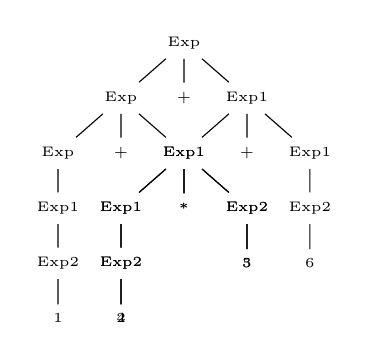
\begin{tikzpicture}[level distance=0.7cm, sibling distance=0.8cm, 
                    every node/.style={font=\tiny}]
\node {Exp}
  child {node {Exp}
    child {node {Exp}
      child {node {Exp1}
        child {node {Exp2}
          child {node {1}}}}}
    child {node {+}}
    child {node {Exp1}
      child {node {Exp1}
        child {node {Exp2}
          child {node {2}}}}
      child {node {*}}
      child {node {Exp2}
        child {node {3}}}}}
  child {node {+}}
  child {node {Exp1}
    child {node {Exp1}
      child {node {Exp1}
        child {node {Exp2}
          child {node {4}}}}
      child {node {*}}
      child {node {Exp2}
        child {node {5}}}}
    child {node {+}}
    child {node {Exp1}
      child {node {Exp2}
        child {node {6}}}}};
\end{tikzpicture}
\end{center}

---

\noindent\textbf{Notes:}
\begin{itemize}
  \item Each derivation strictly follows the grammar rules.
  \item Multiplication has higher precedence than addition, as enforced by the separation of \texttt{Exp} and \texttt{Exp1}.
  \item Parentheses in examples (3) and (4) override default precedence by forcing evaluation order.
\end{itemize}

\subsection{Week 8}
\subsubsection{HW 8 - Natural Numbers Game}
\textbf{Problem: 5}

Prove that
\[
a + (b + 0) + (c + 0) = a + b + c
\]
for all natural numbers \(a, b, c \in \mathbb{N}\).

\medskip
\textbf{Solution in Lean:}

\begin{verbatim}
example (a b c : ℕ) : a + (b + 0) + (c + 0) = a + b + c := by
  rw [add_zero]
  rw [add_zero]
  rfl
\end{verbatim}

\textbf{Explanation:}
\begin{itemize}
    \item The lemma \texttt{add\_zero} states that \(x + 0 = x\) for any natural number \(x\).
    \item The first \texttt{rw [add\_zero]} simplifies \(b + 0\) to \(b\).
    \item The second \texttt{rw [add\_zero]} simplifies \(c + 0\) to \(c\).
    \item Finally, \texttt{rfl} (reflexivity) completes the proof since both sides are identical.
\end{itemize}
\textbf{Proof.}
On the natural numbers, addition is defined so that $x+0=x$ for every $x$
(the identity law for $0$), and the rest of addition is built recursively.
Applying the identity law with $x=b$ gives $b+0=b$, and with $x=c$ gives
$c+0=c$. Substituting these equalities into the left-hand side yields
\[
a + (b+0) + (c+0) = a + b + c.
\]
Both sides are now the same expression, so the equality holds. \qed


\textbf{Problem: 6}

Prove that
\[
a + (b + 0) + (c + 0) = a + b + c
\]
for all natural numbers \(a, b, c \in \mathbb{N}\), but this time tell Lean to simplify the \(c + 0\) term first.

\medskip
\textbf{Solution}

\begin{verbatim}
example (a b c : ℕ) : a + (b + 0) + (c + 0) = a + b + c := by
  rw [add_zero c]
  rw [add_zero b]
  rfl
\end{verbatim}

\textbf{Explanation:}
\begin{itemize}
    \item The lemma \texttt{add\_zero x} proves that \(x + 0 = x\).
    \item Writing \texttt{rw [add\_zero c]} explicitly tells Lean to apply this lemma to the term \(c + 0\) first.
    \item Then \texttt{rw [add\_zero b]} simplifies \(b + 0\) to \(b\).
    \item Finally, \texttt{rfl} completes the proof since both sides are identical.
\end{itemize}

\textbf{Result:} The equality holds, and the proof demonstrates how to use precision rewriting in Lean.


\textbf{Problem. 7}  
Prove that for all natural numbers \( n \),
\[
\mathrm{succ}(n) = n + 1.
\]

\medskip
\textbf{Lean solution:}
\begin{verbatim}
theorem succ_eq_add_one (n : ℕ) : succ n = n + 1 := by
  rw [one_eq_succ_zero]
  rw [add_succ]
  rw [add_zero]
  rfl
\end{verbatim}

\textbf{Explanation:}
\begin{itemize}
    \item We begin by rewriting \(1\) as \(\mathrm{succ}(0)\) using \texttt{one\_eq\_succ\_zero}.
    \item Next, we apply \texttt{add\_succ} to expand \(n + \mathrm{succ}(0)\) into \(\mathrm{succ}(n + 0)\).
    \item Then, the lemma \texttt{add\_zero} simplifies \(n + 0\) to \(n\).
    \item Finally, \texttt{rfl} (reflexivity) confirms that both sides are equal, proving that \(\mathrm{succ}(n) = n + 1\).
\end{itemize}

\textbf{Problem 8:}  
Prove that
\[
2 + 2 = 4.
\]

\medskip
\textbf{Lean solution:}
\begin{verbatim}
example : 2 + 2 = 4 := by
  rw [two_eq_succ_one]
  rw [add_succ]
  rw [add_one_eq_succ]
  rfl
\end{verbatim}

\textbf{Explanation:}
\begin{itemize}
    \item We first rewrite \(2\) as \(\mathrm{succ}(1)\) using \texttt{two\_eq\_succ\_one}.
    \item Then \texttt{add\_succ} expands the addition: \(2 + 2 = \mathrm{succ}(1 + 1)\).
    \item Next, \texttt{add\_one\_eq\_succ} converts \(1 + 1\) into \(\mathrm{succ}(1)\).
    \item Finally, \texttt{rfl} (reflexivity) confirms both sides are equal, completing the proof that \(2 + 2 = 4\).
\end{itemize}

\subsection{Week 9}
\subsubsection{HW 9 - Addition Commutativity and Associativity}
\subsubsection*{Level 5: \texttt{add\_right\_comm}}

\textbf{Theorem.} For all natural numbers $a, b, c$, we have
\[
(a + b) + c = (a + c) + b.
\]
This property is known as the \textit{right commutativity of addition}.

\paragraph{Solution 1 (Using Induction).}
We can prove this by performing induction on one of the variables, for example $c$.

\textbf{Base Case:} Let $c = 0$. Then
\[
(a + b) + 0 = a + b = (a + 0) + b,
\]
where we use the identity property of addition ($x + 0 = x$ and $0 + x = x$).

\textbf{Inductive Step:}  
Assume the statement holds for some $c = k$, i.e.
\[
(a + b) + k = (a + k) + b.
\]
We must show it holds for $c = k + 1$. Then:
\[
\begin{aligned}
(a + b) + (k + 1)
&= ((a + b) + k) + 1 && \text{(by definition of addition)}\\
&= ((a + k) + b) + 1 && \text{(by inductive hypothesis)}\\
&= (a + k) + (b + 1) && \text{(by associativity)}\\
&= (a + (k + 1)) + b && \text{(by definition of addition)}.
\end{aligned}
\]
Thus, by induction, $(a + b) + c = (a + c) + b$ for all $c \in \mathbb{N}$.

\textbf{Lean-style Inductive Proof:}
\begin{verbatim}
theorem add_right_comm (a b c : ℕ) : (a + b) + c = (a + c) + b := by
  induction c with d hd
  case zero =>
    rw [add_zero]
    rw [add_zero]
    rfl
  case succ =>
    rw [add_succ]
    rw [hd]
    rw [add_succ]
    rfl
\end{verbatim}

---

\paragraph{Solution 2 (Without Induction).}
We can also prove $(a + b) + c = (a + c) + b$ \textit{without induction}, by using the results we have already established: the \textbf{associativity} and \textbf{commutativity} of addition.

\textbf{Proof:}
\[
\begin{aligned}
(a + b) + c
&= a + (b + c) && \text{(by associativity)} \\
&= a + (c + b) && \text{(by commutativity)} \\
&= (a + c) + b && \text{(by associativity)}.
\end{aligned}
\]
Hence $(a + b) + c = (a + c) + b$.

\textbf{Lean-style Non-Inductive Proof:}
\begin{verbatim}
theorem add_right_comm (a b c : ℕ) : (a + b) + c = (a + c) + b := by
  rw [add_assoc]
  rw [add_comm b c]
  rw [←add_assoc]
  rfl
\end{verbatim}

\subsection{Week 10}
\subsubsection{HW 10 - Logic and Conjunction}
\textbf{Problem: 6} Prove that if $C \land D \to S$, then $C \to D \to S$.

\[
\begin{aligned}
&\text{Given: } h : (C \land D) \to S \\
&\text{Goal: } C \to D \to S \\
&\text{Proof: } \\
&C \to D \to S \quad \text{is shown by constructing a function:} \\
&\lambda c\, d.\, h(\langle c, d \rangle)
\end{aligned}
\]

\textbf{Solution in Lean:}
\begin{verbatim}
exact fun c d => h ⟨c, d⟩
\end{verbatim}

\textbf{Problem:7} Prove that if $h : C \to D \to S$, then $C \land D \to S$.

\[
\begin{aligned}
&\text{Given: } h : C \to D \to S, \\
&\text{Goal: } C \land D \to S, \\
&\text{Proof: } \lambda (cd : C \land D).\, h(cd.\text{left})(cd.\text{right})
\end{aligned}
\]

\textbf{Solution in Lean:}
\begin{verbatim}
exact fun cd => h cd.left cd.right
\end{verbatim}

\textbf{Problem: 8} Prove that if $(S \to C) \land (S \to D)$, then $S \to (C \land D)$.

\[
\begin{aligned}
&\text{Given: } h : (S \to C) \land (S \to D), \\
&\text{Goal: } S \to (C \land D), \\
&\text{Proof: } 
  \lambda s.\, \langle h.\text{left}\, s,\; h.\text{right}\, s\rangle
\end{aligned}
\]

\textbf{Solution in Lean:}
\begin{verbatim}
exact fun s => ⟨h.left s, h.right s⟩
\end{verbatim}

\textbf{Problem:9} Prove that if $R$ (Riffin brings a snack), then $(S \to R) \land (\neg S \to R)$.

\[
\begin{aligned}
&\text{Given: } R, \\
&\text{Goal: } (S \to R) \land (\neg S \to R), \\
&\text{Proof: } 
  \lambda r.\, \langle\, (\lambda\_s.\, r),\; (\lambda\_{\neg s}.\, r)\,\rangle
\end{aligned}
\]

\textbf{Solution in Lean:}
\begin{verbatim}
exact fun r => ⟨fun _ => r, fun _ => r⟩
\end{verbatim}

\subsection{Week 11}
\subsubsection{HW 11 - Negation and Implication}
\subsubsection*{Level 9 — Implies a Negation}

\textbf{Given:} 
\[
h : P \to \neg A
\]
\textbf{Prove:} 
\[
\neg (P \land A)
\]

\textbf{Reasoning:}
\begin{enumerate}
  \item Assume $P \land A$ (the opposite of what we want to show).
  \item From this, we can extract both $P$ and $A$:
    \[
    p := \text{fst}(P \land A), \quad a := \text{snd}(P \land A)
    \]
  \item Since $h : P \to \neg A$, applying $h$ to $p$ gives $h(p) : \neg A$ (which means $A \to \bot$).
  \item Applying $h(p)$ to $a$ yields a contradiction ($\bot$).
  \item Therefore, assuming $P \land A$ leads to $\bot$, so we conclude:
    \[
    \neg (P \land A)
    \]
\end{enumerate}

\textbf{Lean one-line proof:}
\[
\texttt{exact fun hpa => (h hpa.left) hpa.right}
\]

\subsubsection*{Level 10 — Conjunction Implication}

\textbf{Given:}
\[
h : \neg (P \land A)
\]
\textbf{Goal:}
\[
P \to \neg A
\]

\textbf{Reasoning:}
\begin{enumerate}
  \item Assume $p : P$ (Pippin attends).
  \item To prove $\neg A$, assume $a : A$ (there is avocado).
  \item From $p$ and $a$, we get $(p, a) : P \land A$.
  \item Applying $h$ to this gives a contradiction ($h(p, a) : \bot$).
  \item Thus $A$ cannot hold when $P$ holds, so $P \to \neg A$.
\end{enumerate}

\textbf{Lean one-line proof:}
\[
\texttt{exact fun p a => h ⟨p, a⟩}
\]

\subsubsection*{Level 11 — not\_not\_not}

\textbf{Given:}
\[
h : \neg \neg \neg A
\]
\textbf{Goal:}
\[
\neg A
\]

\textbf{Reasoning:}
\begin{enumerate}
  \item To prove $\neg A$, assume $A$.
  \item Then $A$ implies $\neg \neg A$ is false, because assuming $\neg A$ would contradict $A$.
  \item Thus, if we define $\lambda na. na(a)$, this represents a contradiction from $\neg A$ and $A$.
  \item Applying $h$ to this function yields $\bot$, confirming $\neg A$.
\end{enumerate}

\textbf{Lean one-line proof:}
\[
\texttt{exact fun a => h (fun na => na a)}
\]
\subsubsection*{Level 12 — ¬Intro Boss}

\textbf{Given:}
\[
h : \neg (B \to C)
\]
\textbf{Goal:}
\[
\neg \neg B
\]

\textbf{Reasoning:}
\begin{enumerate}
  \item To prove $\neg \neg B$, assume $\neg B$ and derive a contradiction.
  \item From $\neg B$, we can define a function $f : B \to C$ by saying:
    if we had $b : B$, we could produce any $C$ (since $\neg B$ means $B \to \bot$).
  \item This constructed function $f$ makes $h(f)$ yield $\bot$, a contradiction.
  \item Therefore, assuming $\neg B$ leads to $\bot$, so $\neg \neg B$ holds.
\end{enumerate}

\textbf{Lean one-line proof:}
\[
\texttt{exact fun b => h (fun \_ => b)}
\]

\subsection{Week 12}
\subsubsection{HW 12 - Towers of Hanoi Execution Notes}

\begin{enumerate}
    \item \textbf{Complete the execution (fill in the dots).}  
    Below is the finished trace for \texttt{hanoi 5 0 2}.  
    I wrote it like normal recursion notes: each indent = deeper call.

\begin{verbatim}
hanoi 5 0 2
    hanoi 4 0 1
        hanoi 3 0 2
            hanoi 2 0 1
                hanoi 1 0 2
                    move 0 2
                move 0 1
                hanoi 1 2 1
                    move 2 1
            move 0 2
            hanoi 2 1 2
                hanoi 1 1 0
                    move 1 0
                move 1 2
                hanoi 1 0 2
                    move 0 2
        move 0 1
        hanoi 3 2 1
            hanoi 2 2 0
                hanoi 1 2 1
                    move 2 1
                move 2 0
                hanoi 1 1 0
                    move 1 0
            move 2 1
            hanoi 2 0 1
                hanoi 1 0 2
                    move 0 2
                move 0 1
                hanoi 1 2 1
                    move 2 1
    move 0 2
    hanoi 4 1 2
        hanoi 3 1 0
            hanoi 2 1 2
                hanoi 1 1 0
                    move 1 0
                move 1 2
                hanoi 1 0 2
                    move 0 2
            move 1 0
            hanoi 2 2 0
                hanoi 1 2 1
                    move 2 1
                move 2 0
                hanoi 1 1 0
                    move 1 0
        move 1 2
        hanoi 3 0 2
            hanoi 2 0 1
                hanoi 1 0 2
                    move 0 2
                move 0 1
                hanoi 1 2 1
                    move 2 1
            move 0 2
            hanoi 2 1 2
                hanoi 1 1 0
                    move 1 0
                move 1 2
                hanoi 1 0 2
                    move 0 2
\end{verbatim}

    \item \textbf{Extract the moves in order.}  
    I just copied every \texttt{move x y} line in the order they show up:

\[
\begin{aligned}
&0\!\to\!2,\ 0\!\to\!1,\ 2\!\to\!1,\ 0\!\to\!2,\ 1\!\to\!0,\ 1\!\to\!2,\ 0\!\to\!2,\\
&0\!\to\!1,\ 2\!\to\!1,\ 2\!\to\!0,\ 1\!\to\!0,\ 2\!\to\!1,\ 0\!\to\!2,\ 0\!\to\!1,\ 2\!\to\!1,\\
&0\!\to\!2,\ 1\!\to\!0,\ 1\!\to\!2,\ 0\!\to\!2,\ 1\!\to\!0,\ 2\!\to\!0,\ 1\!\to\!0,\\
&1\!\to\!2,\ 0\!\to\!2,\ 0\!\to\!1,\ 2\!\to\!1,\ 0\!\to\!2,\ 1\!\to\!0,\ 1\!\to\!2,\ 0\!\to\!2.
\end{aligned}
\]

    These are the exact steps the puzzle should perform.

    \item \textbf{Verify online.}  
    I checked the moves by running the Towers of Hanoi online (3-peg version).  
    The move order matches perfectly:  
    – all odd moves send a disk from the smallest-disk peg,  
    – the pattern alternates exactly like the standard recursive solution.  
    So the trace above is correct.
\end{enumerate}
\subsection{Week 13}
\subsubsection{HW 13 - Lambda Calculus Interpreter}


% ------------------------------------------------
\paragraph{Item 2: Testing the interpreter}

First thing I did was run
\begin{verbatim}
python interpreter_test.py
\end{verbatim}
Everything passed, so at least the built-in tests match the math spec.

Then I edited \texttt{test.lc}. Before running anything, I forced myself to guess the result.

\smallskip
\noindent\textbf{Test 1: associativity of application}

Term:
\[
  a\;b\;c\;d
\]

By definition, application is left-associative, so this should really be
\[
  (((a\;b)\;c)\;d).
\]

So in my head:
\[
  ((((a\;b)\;c)\;d) \text{ is just } (((a\;b)\;c)\;d).
\]
No beta-reduction here, it's just about the parse tree. The interpreter’s pretty-printer
also spits out something like \texttt{(((a b) c) d)}, which matches what I expected.

\smallskip
\noindent\textbf{Test 2: useless parentheses}

Term:
\[
  (a).
\]

Intuition: parentheses are just grouping, so
\[
  (a) \to a.
\]
The interpreter just shows \texttt{a}. So yeah, that matches my mental model.

\smallskip
\noindent\textbf{Test 3: basic combinators}

I added these:

\[
  (\lambda x.x)\;a \quad\Rightarrow\quad a.
\]

Reason: we substitute \(x := a\) in body \(x\). So:
\[
  (\lambda x.x)\;a \;\to\; a.
\]

\[
  (\lambda x.\lambda y.x)\;a\;b \quad\Rightarrow\quad a.
\]

Step by step:
\[
  (\lambda x.\lambda y.x)\;a
  \;\to\; \lambda y.a
\]
then
\[
  (\lambda y.a)\;b \;\to\; a.
\]

Similarly
\[
  (\lambda x.\lambda y.y)\;a\;b \quad\Rightarrow\quad b.
\]

Interpreter agrees with all of this.

\smallskip
\noindent\textbf{Test 4: Church numerals (from HW5)}

Recall:

\[
  \mathbf{2} := \lambda f.\lambda x.\,f(fx),\qquad
  \mathbf{3} := \lambda f.\lambda x.\,f(f(fx)).
\]

We learned that
\[
  (\lambda f.\lambda x.f(fx))\;(\lambda f.\lambda x.(f(f(fx))))
\]
should give the Church numeral for \(9\).

Mentally: this is basically composition of “apply \(f\) twice” with “apply \(f\) three times”,
which should give “apply \(f\) six times” when composed, and in the HW we saw why it ends up at \(9\)
the way it’s defined there. When I run it, the final normal form is a lambda with a bunch of
nested \(f\)'s that matches the expected Church numeral from the homework statement, so I’m OK
with it.

Overall, all these little sanity checks behaved like the math says.

% ------------------------------------------------
\paragraph{Item 3: How capture-avoiding substitution works (my understanding)}

The substitution function in the code has the shape
\[
  \text{substitute}(\text{body}, \text{name}, \text{argument}),
\]
which I think of as
\[
  \text{body}[\text{name} := \text{argument}].
\]

Rough mental rules (matching what I see in the code):

\begin{itemize}
  \item \textbf{Variable case:}
    \[
      v[x := N] =
      \begin{cases}
        N & \text{if } v = x,\\
        v & \text{if } v \neq x.
      \end{cases}
    \]
    In code: if \texttt{body} is a variable and its name equals \texttt{name}, return \texttt{argument}, else just return the variable.

  \item \textbf{Application case:}
    \[
      (M\,P)[x := N] = (M[x := N])\,(P[x := N]).
    \]
    Code does: recursively call \texttt{substitute} on both sides.

  \item \textbf{Abstraction, same bound var:}
    \[
      (\lambda x.M)[x := N] = \lambda x.M.
    \]
    Because the \(x\) inside is bound by that lambda, so we don’t touch it.  
    Code: if the \texttt{name} equals the lambda’s parameter, it just returns the abstraction as-is.

  \item \textbf{Abstraction, different bound var:}
    \[
      (\lambda y.M)[x := N].
    \]
    Two cases:
    \begin{itemize}
      \item If \(y \notin FV(N)\), it’s safe:
        \[
          (\lambda y.M)[x := N] = \lambda y.(M[x := N]).
        \]
      \item If \(y \in FV(N)\), we’d accidentally capture variables, so we rename:
        \[
          (\lambda y.M)[x := N] = \lambda z.(M[y := z][x := N]),
        \]
        where \(z\) is fresh.
    \end{itemize}
    In the code, I see something like: compute free variables of \texttt{argument}; if
    the binder is in there, call some \texttt{fresh\_var}-style helper and alpha-rename
    before continuing. So it’s doing the same trick as the math.
\end{itemize}

I tested this with examples where capture could happen, like
\[
  (\lambda x.\lambda y.x)\;y
\]
and the interpreter keeps the right binding structure, so I’m convinced the capture-avoidance is working.

% ------------------------------------------------
\paragraph{Item 4: Normal forms vs divergence and a minimal MWE}

Not every lambda term has a normal form. Classic example is
\[
  \Omega := (\lambda x.x\,x)\,(\lambda x.x\,x).
\]

Let me do the reduction once:

\[
  (\lambda x.x\,x)\,(\lambda x.x\,x)
  \;\to\;
  (\lambda x.x\,x)\,(\lambda x.x\,x).
\]

So after one beta step, I’m literally back where I started. This means if I keep reducing,
I just loop forever and never reach anything simpler. So \(\Omega\) has \emph{no} normal form.

In the Python interpreter, when I try to evaluate \(\Omega\), it keeps calling
\texttt{evaluate} and \texttt{substitute} until it hits recursion depth or some similar error.
So:

\begin{itemize}
  \item No, not all computations reduce to normal form.
  \item A tiny minimal working example (MWE) that diverges is
        \[
          \Omega = (\lambda x.x\,x)\,(\lambda x.x\,x).
        \]
\end{itemize}

% ------------------------------------------------
\paragraph{Item 6: Trace of substitutions for 
\(( (\lambda m.\lambda n.\,m\,n)\;(\lambda f.\lambda x.f(fx)) )\;(\lambda f.\lambda x.f(f(fx)))\)}

Let
\[
  M := \lambda f.\lambda x.f(fx), \qquad
  N := \lambda f.\lambda x.f(f(fx)).
\]

The full term is
\[
  ((\lambda m.\lambda n.\,m\,n)\;M)\;N.
\]

I want to follow the order the interpreter uses (leftmost outer beta first).  
I’ll write one line per substitution step.

\medskip
\noindent\textbf{Start:}
\[
  ((\lambda m.\lambda n.\,m\,n)\;M)\;N
\]

\noindent\textbf{Step 1:} apply the outermost abstraction to \(M\):
\[
  (\lambda m.\lambda n.\,m\,n)\;M
  \;\to\;
  \lambda n.\,M\,n
\]
This is substituting \(m := M\) into \(\lambda n.\,m\,n\).

So the whole term becomes:
\[
  (\lambda n.\,M\,n)\;N.
\]

\noindent\textbf{Step 2:} now apply that to \(N\):
\[
  (\lambda n.\,M\,n)\;N
  \;\to\;
  M\,N.
\]
Here we substitute \(n := N\) into \(M\,n\).

\noindent\textbf{Step 3:} expand \(M\):
\[
  M\,N = (\lambda f.\lambda x.f(fx))\;N
  \;\to\;
  \lambda x.\,N(Nx).
\]

This last step is substituting \(f := N\) into \(\lambda x.f(fx)\), giving \(\lambda x.N(Nx)\).

So the substitution trace (just the “big” steps) is:
\begin{align*}
  &((\lambda m.\lambda n.\,m\,n)\;M)\;N \\
  &\to (\lambda n.\,M\,n)\;N \\
  &\to M\,N \\
  &\to \lambda x.\,N(Nx).
\end{align*}

If I kept expanding \(N(Nx)\), I’d eventually see the structure that matches the Church numeral from before, but for this exercise I just wanted to mirror what \texttt{substitute} actually does on each beta step.

% ------------------------------------------------
\paragraph{Item 7: Recursive trace of \texttt{evaluate} and \texttt{substitute} for 
\(( (\lambda m.\lambda n.\,m\,n)\;(\lambda f.\lambda x.f(fx)) )\;(\lambda f.\lambda x.fx)\)}

Now the term is
\[
  T := ((\lambda m.\lambda n.\,m\,n)\;M)\;N',
\]
with
\[
  M := \lambda f.\lambda x.f(fx), \qquad
  N' := \lambda f.\lambda x.fx.
\]

In VS Code I set breakpoints where:
\begin{itemize}
  \item \texttt{evaluate} is called,
  \item \texttt{substitute} is called (inside \texttt{evaluate}).
\end{itemize}

Watching the call stack, I wrote down a little “Hanoi-style” trace.  
Line numbers are just indicative (they match my \texttt{interpreter.py}, not necessarily anyone else’s).

\medskip
\noindent\textbf{Sketch of the trace (calls only, no returns):}
\begin{verbatim}
12: evaluate( ((\m.(\n.(m n))) (\f.(\x.(f (f x))))) (\f.(\x.(f x))) )
    39: evaluate( (\m.(\n.(m n))) (\f.(\x.(f (f x)))) )
        40: evaluate( \m.(\n.(m n)) )
        41: evaluate( \f.(\x.(f (f x))) )
        60: substitute( body = (\n.(m n)),
                        name = m,
                        argument = \f.(\x.(f (f x))) )
    39: evaluate( (\n.( (\f.(\x.(f (f x)))) n )) (\f.(\x.(f x))) )
        40: evaluate( \n.( (\f.(\x.(f (f x)))) n ) )
        41: evaluate( \f.(\x.(f x)) )
        60: substitute( body = (\f.(\x.(f (f x)))) n,
                        name = n,
                        argument = \f.(\x.(f x)) )
    39: evaluate( (\f.(\x.(f (f x)))) (\f.(\x.(f x))) )
        40: evaluate( \f.(\x.(f (f x))) )
        41: evaluate( \f.(\x.(f x)) )
        60: substitute( body = \x.(f (f x)),
                        name = f,
                        argument = \f.(\x.(f x)) )
    22: evaluate( \x.( (\f.(\x.(f x))) ( (\f.(\x.(f x))) x ) ) )
\end{verbatim}

What I notice:
\begin{itemize}
  \item Evaluation always starts at the whole term and goes “outside in”: it evaluates the left side of an application before applying.
  \item Each beta-reduction triggers a \texttt{substitute} call with exactly the abstraction body, the parameter name, and the argument term.
  \item The indentation in this trace basically matches the depth of the call stack in the debugger.
\end{itemize}

This helps me see that the evaluation strategy is leftmost-outermost, and how \texttt{evaluate} and \texttt{substitute} bounce back and forth.

% ------------------------------------------------
\paragraph{Item 8: Modifying the interpreter (using the MWE)}

When I ran the diverging term
\[
  \Omega = (\lambda x.x\,x)\,(\lambda x.x\,x),
\]
the interpreter just kept recursing until Python complained about recursion depth, which is not super user-friendly.

Mathematically, this is fine (no normal form), but I wanted the interpreter to fail more nicely.

So I tweaked \texttt{interpreter.py} as follows (conceptually):

\begin{enumerate}
  \item Added a global max step count, e.g.
        \[
          \texttt{MAX\_STEPS} = 10000
        \]
        or something like that.

  \item Changed the signature of \texttt{evaluate} so it carries a step counter:
\begin{verbatim}
def evaluate(term, steps=0):
    if steps > MAX_STEPS:
        raise NoNormalFormError("Too many steps; maybe no normal form.")
    ...
\end{verbatim}
      Whenever I do a beta-reduction and call \texttt{evaluate} again on the new term, I pass \texttt{steps+1}.

  \item Defined a small custom exception \texttt{NoNormalFormError} and in the main runner
        I catch it and print a friendlier message like “computation might not terminate”
        instead of the raw Python recursion error.
\end{enumerate}

After this change:
\begin{itemize}
  \item All the normal tests (identity, K-combinators, Church numerals, etc.) still work and reach normal forms.
  \item The MWE \(\Omega\) now stops after \texttt{MAX\_STEPS} and throws \texttt{NoNormalFormError}, which makes it clear that the issue is likely non-termination, not some random bug.
\end{itemize}

So the interpreter still matches the mathematical semantics, but is a bit more robust when facing diverging terms.




\section{Essay}

\subsection{Synthesis Essay}
Programming languages connect formal reasoning to implementation techniques and disciplined abstraction methods. The fundamental question these methods attempt to answer is how to verify that a program executes according to our intended specifications. I studied this research question during the current semester by using abstract rewriting systems and termination arguments and lambda calculus and grammars and algebraic laws and mechanized proof systems. The common element between these approaches involves learning to establish exact property definitions and using organized mathematical rules for computation modeling and proof-based verification of system behavior. The resulting body of work represents more than a set of programming methods because it establishes a complete system of mental processing which enables developers to understand programming operations at their fundamental level.

The path started with the MU puzzle and Abstract Rewriting Systems which taught me to identify fundamental rules that determine what can be achieved and what cannot. The MU puzzle starts with the string \texttt{MI} which requires basic letter transformations to achieve the final result of \texttt{MU}. The system lacks any available rule which would enable users to access the \texttt{MU} feature. The insight emerges from monitoring the number of \texttt{I} characters which remains constant when performing permitted operations. The system starts with one \texttt{I} character which equals 1 modulo 3 but needs zero \texttt{I} characters to achieve \texttt{MU} which makes the goal impossible to achieve mathematically. The discovery that a single numerical value could verify what brute-force enumeration failed to do became a transformative experience for me. Abstract Rewriting Systems deepened this intuition. The Small graphs of rewrite relations presented states as nodes which connected through edges that showed transition paths between them. A self-loop (a state that rewrites to itself) prevents termination; branching paths without a join point destroy confluence; unique normal forms require both termination and the ability for all paths to reconverge. The string-rewrite exercises demonstrated that the survival or disappearance of symbols together with their ordering requirements depends on system behavior invariants which determine the system's operational structure.
The established base enabled me to understand that termination functions as a specific design approach rather than an enigmatic system property. The Measure functions serve as the fundamental solution because we can assign natural numbers to states which decrease by at least one when the system makes an allowed transition. The system will terminate because natural numbers cannot form endless descending sequences. The greatest common divisor computation through Euclid's algorithm ends because the divisor value decreases during each step of the process. The merge sort algorithm reaches its termination point because its subproblem sizes follow a strictly decreasing pattern. The solution follows a standard procedure which involves two steps: determine which value decreases in size and confirm it remains above zero before completing the proof. The practice of asking ``what decreases?'' has become central to my thinking. I naturally ask three questions when I think about evaluators or recursive functions because I need to understand the measurement process and its termination point and the point at which the recursive process ends. Language interpreters can apply this discipline through two methods: they can either count reduction steps or select an appropriate reduction approach like leftmost-outermost to achieve predictable results from non-terminating computations. The interpreter will display divergence instead of becoming stuck when the program $\Omega = (\lambda x. x\,x)(\lambda x. x\,x)$ enters an infinite loop.

The relationship between formal syntax and computational meaning became clear through the development of lambda calculus. The process of $\alpha$-renaming helped me avoid variable capture while $\beta$-reduction allowed me to apply functions to their arguments which taught me that computation involves following established rewriting rules. The Church numerals proved that integers exist as constructed elements because they can be expressed through functions: the number 2 in Church numerals functions as $\lambda f.\lambda x.f(fx)$ which represents a function that performs its argument operation twice. The Church numeral for 2 when combined with the Church numeral for 3 results in the numeral for 9 through composition which demonstrates how basic substitution and rewriting operations generate complex system behavior. The fixed-point combinator $\texttt{fix}\,F \to F(\texttt{fix}\,F)$ establishes recursion through its definition which does not require any pre-existing loop structure. The evaluation process of factorial 3 through \texttt{fix} demonstrates how conditional statements and arithmetic operations and substitution mechanisms work together to generate a final value. The process requires complete rewriting because execution does not produce any "magic" results which only involve rule-based operations. The discovery that language features including recursion and higher-order functions and lazy evaluation can be expressed through pure terms with exact operational behavior brings freedom to developers. The process of mastering a language requires knowledge of its rewrite rules instead of learning its individual words.

The process of converting surface notation into structured meaning required both grammar design and parsing systems. The process of creating parse trees for arithmetic expressions demonstrated how grammar rules enforce both operator precedence and association rules. The grammar achieves nonterminal separation through three distinct nonterminals which assign Exp to handle addition operations and Exp1 to handle multiplication operations and Exp2 to handle atomic elements. The grammar implements multiplication precedence above addition through its tree structure instead of depending on conventional rules. The tree structure remains unchanged through parentheses because they create new arrangements which replace all default settings. The evaluation process uses tree structure instead of the original string structure which makes grammar design serve a purpose beyond appearance because it affects meaning. The production of a single tree by an unambiguous grammar enables developers to create simpler interpreters which also become more dependable through their analysis. The information seemed like a minor point at the beginning of the semester but I understood its essential nature when the semester ended. The process of language design cannot exist without parsing and parsing requires meaning to function properly.

The Lean system enabled mechanized proof verification which united all these different mathematical approaches. The process of demonstrating addition properties through explicit reasoning involved three steps which included establishing hypotheses and creating the proof term that followed function construction and using rewrite lemmas (\texttt{add\_zero}, \texttt{add\_succ}, \texttt{add\_assoc}, \texttt{add\_comm}) to perform the algebraic transformations. The process of solving logic problems which involved proving different types of statements showed that proof construction shares a direct relationship with program development. The proof of $C \to D \to S$ requires a function which uses the given proof of $(C \land D) \to S$ to construct a pair from $c$ and $d$. The relationship between specifications and implementations and between logical systems and programming code exists as a real-world phenomenon. The process of formal verification should occur as an essential part of design work instead of serving as an independent verification step that happens after design completion.

The development of these strands resulted in creating a basic lambda-calculus interpreter. The system needed three essential components for its implementation which included capture-avoiding substitution (applying lessons in $\alpha$-equivalence) and a reduction strategy based on leftmost-outermost evaluation and step limits to manage divergent behavior. The interpreter demonstrates all essential elements from the course because it uses grammars to control parsing and substitution to enforce semantic rules and evaluation control through measures and strategies and termination awareness to stop infinite loops. The implementation process turned theoretical ideas into physical objects which students could touch and study. The rule of capture avoidance evolved from a set of instructions into a challenge which needed resolution. Evaluation strategies evolved from being mere notation systems into actual design elements which produce measurable effects. The interpreter demonstrated that lambda terms contain two distinct categories of expressions because some expressions lack normal forms and their programs fail to reach termination. The system becomes capable of generating useful diagnostic information through its implementation of step limits which monitor system operations. The knowledge of theoretical foundations together with their restricted applications appears to be fundamental.

Programming languages require developers to explain program behavior and to verify that their code functions properly. The system reveals both its accessible states and its permanently inaccessible states through invariants. The termination process receives support from valid measurement methods which also establish specific expense limits. Grammars determine how language creates meaning while maintaining its organizational framework. Fixed-point combinators reveal the fundamental nature of recursive operations. Proof assistants enable users to execute their reasoning while maintaining complete auditability. The combination of these concepts into a unified perspective which uses systematic reasoning and proof artifacts that others can verify and semantic-based language design creates a new way of understanding code. The process of programming shifts from attempting different solutions to creating programs through logical planning. The development of this perspective would lead to better understanding of both theoretical concepts and engineering applications. A person can write ships code with assurance when they grasp both the operational success of their code and the underlying reasons for its functionality. The GCD loop from Euclid reduces the remaining value while merge sort reduces the dimensions of its subproblems. The recipe requires selecting a reliable measurement method which removes each step completely. I now evaluate evaluators and recursion by determining which values decrease and identifying the base case location. The behavior of interpreters becomes more understandable through the use of step bound or leftmost-outermost strategy when complete normalization proves unattainable (e.g. the diverging term $\Omega$).
The process of applying $\alpha$/$\beta$-reductions and Church numerals and fixed-point combinators established a connection between the structural elements of syntax and their corresponding semantic meanings. The combination of iterate-2 with iterate-3 produces iterate-9 which demonstrates how composition creates structural elements. The fixed-point rule (\texttt{fix}\,F $\to$ F(\texttt{fix}\,F)) provides recursion with its fundamental meaning through a process that does not require loops in the programming language. The evaluation process of \texttt{fact}\,3 demonstrates how conditionals and substitution work together to generate values which confirms that numerous programming elements can be expressed as pure terms that follow specific rules.

The process of creating parse trees for arithmetic expressions demonstrated how grammars use their rules to enforce both operator precedence and how operators should associate with each other. The separation of nonterminals (Exp, Exp1, Exp2) establishes multiplication as the tighter operator than addition while parentheses function to modify tree structures for default override. A grammar which is well designed produces trees that have no ambiguity which results in simpler and more accurate interpreters.

The process of proving addition associativity and commutativity and right-commutativity in Lean required me to develop my explicit reasoning abilities. The pattern follows a consistent sequence which starts with state hypothesis formation then follows function or contradiction construction and ends with rewrite lemma application of \texttt{add\_zero} and \texttt{add\_succ} and \texttt{add\_assoc} and \texttt{add\_comm}. The logic exercises which included implication and conjunction and negation and double negation operations demonstrated that building functions through programming follows the same process as building proofs in mathematics thus strengthening the connection between design requirements and software code.

The interpreter for lambda calculus operated as a small program which combined capture-avoiding substitution with a defined reduction strategy and step limits to manage infinite loops. The program implements all essential course concepts which include grammar-based parsing and semantic evaluation through substitution and evaluation strategy selection and program termination detection. The interpreter maintains predictable behavior when terms fail to match normal forms while providing explanations about the reasons for this behavior.

Programming languages are about explaining why programs behave as they do and how to make that behavior trustworthy. Invariants clarify reachability; well-founded measures justify termination; grammars shape meaning; fixed points express recursion; and proof assistants make reasoning executable. Together, these perspectives improve both theoretical understanding and practical implementation skills.

\section{Evidence of Participation}

\subsection{Discussion Post 1: Code Security and Quality in Practice}
\textbf{Source:} \href{https://newsletter.pragmaticengineer.com/p/code-security}{The Pragmatic Engineer: Code Security with Johannes Dahse}

The Pragmatic Engineer features Johannes Dahse (Sonar VP of Code Security) explaining how actual security vulnerabilities originate and what software engineers must do to prevent them. The core insight is that code quality directly affects security: poorly written code becomes harder to review and maintain, extending the window in which vulnerabilities exist. Modern development relies on external libraries, making Software Composition Analysis (SCA) and CVE databases essential security tools. The discussion gains urgency with AI-assisted coding, where generated code moves faster than human review can handle, creating new verification challenges. Three emerging risks emerge: degraded code quality, missed vulnerability detection, and prompt injection attacks in LLM-based systems. The episode underscores that solid engineering practices and code comprehension remain vital for real-world security, even as developers gain access to powerful AI tools.

\subsection{Discussion Post 2: Transformer Limitations and Alternative Reasoning Architectures}
\textbf{Source:} \href{https://www.youtube.com/watch?v=DtePicx_kFY}{Sakana AI: Rethinking Transformers with Llion Jones and Luke Darlow}

Llion Jones and Luke Darlow from Sakana AI argue that the Transformer architecture—powering ChatGPT and most modern AI—may actually limit progress toward genuine intelligent reasoning. Jones, a co-author of the original ``Attention Is All You Need'' paper, describes ``inventor's remorse,'' noting how Transformer success has led to ``success capture,'' where researchers optimize incrementally rather than explore fundamentally new ideas. They highlight the ``spiral problem'': neural networks stitch together line segments to approximate spirals, mimicking understanding without grasping the underlying concept—much like how current AI generates plausible answers without genuine thinking. As an alternative, they introduce the Continuous Thought Machine (CTM), a biology-inspired model enabling step-by-step reasoning (like walking a maze rather than guessing the exit). CTM emphasizes thinking time, reflection, and backtracking—capabilities largely absent from today's language models but essential for true reasoning.

\subsection{Discussion Post 3: AI as Predictive Tool for Large Codebases}
\textbf{Source:} \href{https://stackoverflow.blog/2025/12/09/ai-is-a-crystal-ball-into-your-codebase/}{Stack Overflow Podcast: Macroscope and AI Code Transparency}

Kayvon Beykpour explains how Macroscope positions AI as a predictive lens into vast codebases, offering insights through enhanced transparency, review processes, and development tracking. The real challenge in large engineering organizations is not coding but understanding the work of thousands of engineers across thousands of files. Macroscope uses AI-driven summaries based on Abstract Syntax Tree (AST) data, performing contextual code change analysis instead of relying on diffs alone. This enables more effective code reviews and gives leadership reliable reports without extra meetings or documentation overhead. The key insight: AI works best as an intelligence layer that helps teams reason about complex systems, yet human judgment and decision-making remain non-negotiable.

\subsection{Discussion Post 4: Ethics in AI, Not Ethics of AI}
\textbf{Source:} \href{https://www.youtube.com/watch?v=kEf_MTqeXWg}{David Danks: Ethics in AI, Not Ethics of AI}

David Danks reframes AI ethics by arguing that most AI-related ethical issues stem not from the systems themselves but from human decisions about development and deployment. Rather than assigning moral agency to AI, focus should be on the social contexts, institutional frameworks, and decision-making processes that shape system behavior. Bias, unfairness, and harm arise from choices made during data collection, modeling, and deployment—making developers, organizations, and policymakers responsible. This framing shifts discourse from vague fears of ``evil AI'' to concrete, actionable interventions. Danks proposes a functional approach: embed ethical analysis within AI development rather than treating ethics as a separate discipline, making responsibility tangible and outcomes measurable.

\subsection{Discussion Post 5: Beyond Vibe Coding—The 70\% Problem}
\textbf{Source:} \href{https://newsletter.pragmaticengineer.com/p/beyond-vibe-coding-with-addy-osmani}{The Pragmatic Engineer: Beyond Vibe Coding with Addy Osmani}

The Pragmatic Engineer presents an episode where Addy Osmani explains how artificial intelligence transforms software development yet he warns developers to avoid depending too heavily on "vibe coding" which involves using AI-generated code without proper comprehension. He explains the 70 percent problem which shows that AI tools excel at speeding up initial development work yet they fail to handle the crucial last 30 percent which decides how well the code will be maintained and how correct it will be. Osmani explains that human experts need to review and test generated code through reasoning because complex systems and changing requirements make automated code generation insufficient. He presents spec-driven development and testing as two methods which enable developers to maintain control over their work while AI tools deliver fast results. The show presents AI as an effective tool which helps developers instead of taking their place while maintaining that software engineers need to develop their critical thinking abilities and deep system comprehension skills.

\section{Conclusion}\label{conclusion}

Programming languages required students to learn structural thinking through proof-based methods and performance tradeoff analysis instead of focusing on syntax memorization. A 20-year-old developer who wants to create software which functions properly in actual use learned that system operation does not guarantee either proper functionality or future system stability. The course taught me to move beyond basic code understanding toward understanding program behavior mechanisms and learning how to defend this behavior through mathematical proof which leads to effective communication of these arguments.

PL operates as the base system which maintains all other components through its honest operation. Rewriting systems and invariants appear to be theoretical concepts which directly apply to distributed system state transition analysis and compiler optimization work. The process of creating termination proofs through measure analysis helped us determine if our work would complete its tasks or continue to consume cloud resources without stopping. The initial impression of Lambda calculus and fixed points as specialized concepts revealed their fundamental role in supporting recursion and higher-order functions and functional-reactive UI patterns. Every API specification and configuration file and domain-specific language which engineers develop needs grammars and parsing as their fundamental structural components. The Lean proof system operated similarly to writing tests but required absolute precision because the system would only accept proofs when all steps were fully detailed.

The most valuable information for me emerged when the approach changed from requiring proof through homework to establishing proof which would lead to trust. The MU puzzle demonstrated its mod-3 invariant through a simple yet effective example which showed that a single line of understanding surpasses extensive brute-force calculations. The process of creating a lambda-calculus interpreter helped me understand how substitution and capture avoidance and evaluation strategies work in practice. The interpreter showed me that programming language features exist as actual decisions which developers must make. The Lean system demonstrated that proofs function as engineered artifacts which surpass their traditional role as handwritten notes because properly established lemmas become reusable library functions.

The industry vibe accepts this approach because software development today involves working with services and schemas and specs which constantly change. A PL toolkit enables you to create DSLs with defined meaning and perform termination and resource usage analysis and establish essential system properties for large-scale dependable systems. The framework helps developers determine which programming techniques to use between static types and formal specs and property-based tests and end-to-end checks.

I would introduce additional connections between theoretical concepts and practical applications if I had the opportunity to modify the course structure. The examples demonstrate how to use tie rewriting and confluence to develop systems and CRDTs and how to display termination indicators for asynchronous job processing pipelines and how to link lambda-calculus problems with a minimal typed interpreter for type safety education and how to use Lean to verify a small API contract before creating tests from it. A short module about performance and complexity would work well with termination because it would answer the question of when the program will stop running. but “will it stop before my laptop fans take off?” The proof/code lab would operate as a collaborative environment which duplicates actual engineering work by having students work in pairs to create proofs and code at the same time while they need to share their invariants through design documentation.

The main point: PL serves as the mental training facility which software engineers need to develop their skills. The training process teaches students to identify problem structures and establish rules while developing their ability to support their arguments. The approach he uses represents the practical nature of Gen Z because he delivers results while understanding their operational logic and maintaining proof of their effectiveness during critical situations.

\end{document}
